\documentclass[utf8]{article}

\usepackage[utf8]{inputenc}

\usepackage[parfill]{parskip}

\usepackage[T1]{fontenc}
\usepackage[french]{babel}
\usepackage{array,multirow,makecell}
\usepackage{longtable}
\usepackage{setspace}
\usepackage{makecell}
\setcellgapes{1pt}
\makegapedcells
\usepackage[table]{xcolor}
\renewcommand*{\emph}[1]{\textcolor{green}{#1}}
\newcolumntype{R}[1]{>{\raggedleft\arraybackslash }b{#1}}
\newcolumntype{L}[1]{>{\raggedright\arraybackslash }b{#1}}
\newcolumntype{C}[1]{>{\centering\arraybackslash }b{#1}}
\usepackage{amsmath}
\usepackage{amssymb}
\usepackage{amsfonts}
\usepackage{graphicx}
\usepackage{float}
\usepackage{algorithm}
\usepackage{algorithmicx}
\usepackage{algpseudocode}
\usepackage{fullpage}


% -----------------------------------------------------


\title{\\[3 cm]\Huge Software requirements document : \\[1 cm] L-type\\[7 cm]}
\author{ELKENZE Camelia\\[0,2 cm] BARBER Jeremy\\[0,2 cm] Latoundji Salim\\[0,2 cm] DEMIREL Helin\\[0,2 cm] ABDOUL-AZIZ Aïssa\\[0,2 cm] ADEGNON Kokou\\[0,2 cm] KINSOEN Alexandre\\[0,2 cm] VANNESTE Martin\\[0,2 cm] MASSIMETTI Mario  }
\date{20 novembre 2020}

\begin{document}
\tableofcontents

\newpage

% -----------------------------------------------------

\section{Introduction}
Bla bla \emph{bla}.

\subsection{But du projet}
L’objectif de ce projet est de réaliser un shoot them up multijoueur à scrolling vertical dans lequel un ou deux joueurs doivent parcourir plusieurs niveaux en détruisant les ennemis qui se présentent devant eux ainsi qu’en esquivant les salves de tir provoquées par ces derniers.
Les navires de guerre dirigés par les joueurs peuvent récupérer des bonus d’armement lâchés par leurs nombreux adversaires.

\subsection{Glossaire}
Shoot them up : "abattez-les tous", genre de jeu vidéo

\subsection{Historique}
Historique \emph{de notre travail}

\section{Besoins utilisateur}

\subsection{Besoins fonctionnels}

% ajoute de l'image

\begin{figure}[h!]
\centering
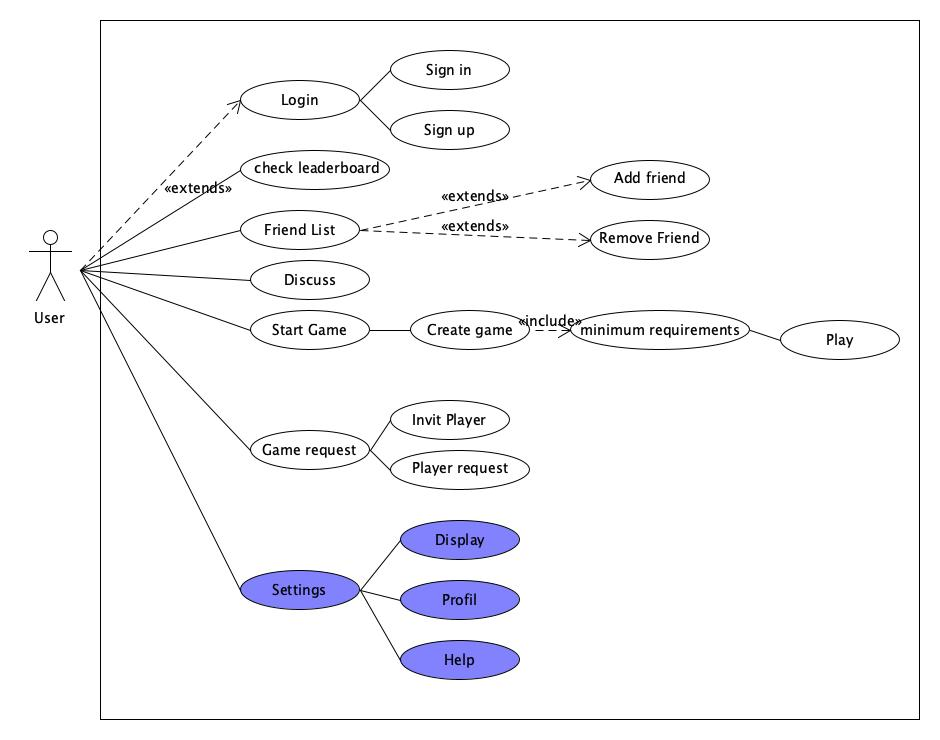
\includegraphics[width=10cm]{UserUseCase1}
\caption{Diagramme de use case coté utilisateur}
\label{fig:UerUseCase}
\end{figure}

\subsubsection{Connexion}
En lançant le programme l'utilisateur arrive sur une page d’accueil qui l'invite à entrer son nom d'utilisateur et son mot de passe si ce dernier possède déjà un compte. 
Si ce n'est pas le cas il a la possibilité de créer un nouveau compte. 
Un pseudo et un mot de passe seront demandés tant que le format des entrées est incorrect et/ou que le pseudo n'est pas unique.
Après s’être connecté l'utilisateur accède automatiquement au menu principal.



\subsubsection{Menu principal}
Une fois l'utilisateur connecté il a accès aux différentes fonctionnalités du jeu telles que:
\begin{itemsize}
\par
\item -Consulter le classement : L'utilisateur peut accéder au classement des meilleurs joueurs du jeu en fonction de leur score.
\item -Consulter sa liste d'amis: La consultation de la liste d'amis se fait sur base
\item -Ajouter un ami: Il est possible de trouver un ami en recherchant son pseudo et de l'ajouter si le pseudo existe. Il n'y a pas de demande d'ajout, si l'utilisateur trouve le second utilisateur leur liste d'amis est automatiquement mise à jour et l'ajout est effectué des deux cotés.
Cépendant si le pseudo n'existe pas un message d'erreur sera renvoyé.
\item-Supprimer un ami: La suppression d'un ami se fait à l'aide du pseudonyme de l'ami en question. Si le pseudo est invalide une erreur sera affichée.
Après la suppression l'ami est retiré de la liste d'ami.
\item-Discuter avec un autre utilisateur : Pour discuter avec un utilisateur il suffit d'entrer son pseudonyme, si le pseudo est connu du programme une fenêtre s'ouvre avec le chat en cours. Toutefois un pseudo invalide engendre un message d'erreur.
En cas d'envoi d'un message à un utilisateur non connecté, le message s'enverra et le destinataire et pourra le lire à sa prochaine connexion.
\item-Envoyer une demande de jeu : L'utilisateur a la possibilité d'inviter un autre utilisateur, avec un pseudo valide, à rejoindre une partie. Si ce dernier est connecté et qu'il n'est pas déjà entrain de jouer, il a possibilité d'accepter ou de refuser la demande. S'il accepte la connexion entre les deux joueurs sera établie, s'il refuse l'hôte ne sera pas averti.
\item-Consulter les demandes de jeu :
Lors d'une consultation de la liste d'invitations, la possibilité est laissée à l'utilisateur d'accepter ou de décliner l'invitation dans le cas ou une invitation est présente dans la liste. Ainsi, accepter une invitation transfère l'utilisateur dans le lobby de l'hôte si ce lobby n'a pas atteint son nombre maximum de joueurs.
L'invité ne peut pas modifier les paramètres que le premier joueur aura choisi.
A l'inverse refuser une invitation n'avertit pas l'hôte. 
\item-Lancer une partie : Le lancement d'une partie se fait lorsque l'utilisateur crée une partie en gardant les paramètres par défauts ou en les redéfinissants.
\end{itemsize}


\subsubsection{Création de partie}
La création d'une partie est une option qui envoie l'utilisateur vers une fenetre de personnalisation permettant de modifier les paramètres du jeu.
Cette fenetre contient déjà des paramètres par défauts.
S'il le souhaite l'utilisateur peut définir :
\begin{itemsize}
\par
\item-Le nombre de joueur:Un joueur a la possibilité de choisir entre un ou deux participants.Dans le cas où le nombre de participants équivaut à deux il aura la possibilité d'entrer un pseudo valide et la partie ne se lancera que si le joueur invité accepte la demande de jeu.
\item-La difficulté de la partie: Chaque partie est composée de plusieurs niveaux qui auront chacun plusieurs niveaux de difficultés.
\item-La probabilité d'apparation des bonus: L'utilisateur a le choix de gérer la probalité qu'aura un ennemi de lacher un bonus après sa destruction.
\item-Le tir allié:La possibilité d'activer le tir allié ne peut être accordé que dans le cas où le nombre de joueur est supérieur à un.
Dans ce premier scénario le joueur a le droit de choisir s'il souhaite que les projectiles de l'invité soit inoffensifs ou non. Cette option vaut pour les deux joueurs.
\item-Le nombre de vies: Il est laissé à l'utilisateur le choix de posséder jusqu'à cinq vies.
\end{itemsize}

Une fois les paramètres validés,si une demande de jeu à un autre joueur a été envoyée le joueur est dirigé vers une salle d'attente en attendant la réponse du second utilisateur. Faute de quoi, le jeu commence directement.


\subsubsection{Settings}
En entrant dans settings , l'utilisateur a le choix d'accéder à différentes options :
\item-Display : Cette option permettra à l'utilisateur de modifier le style du jeu tel que changer la couleur de l'arrière plan de la partie. (Cette option sera développée d'avantage dans les futures versions)
\item-Profil : En accédant à cette option l'utilisateur a le droit de modifier toutes les informations liées à son compte. Si ces nouvelles informations sont valides le profil sera mis à jour.
\item-Help: Cette section permet à l'utilisateur de consulter les règles du jeu s'il le souhaite.


\section{Besoins système}
\subsection{Besoins fonctionnels}
\begin{figure}[h!]
\centering
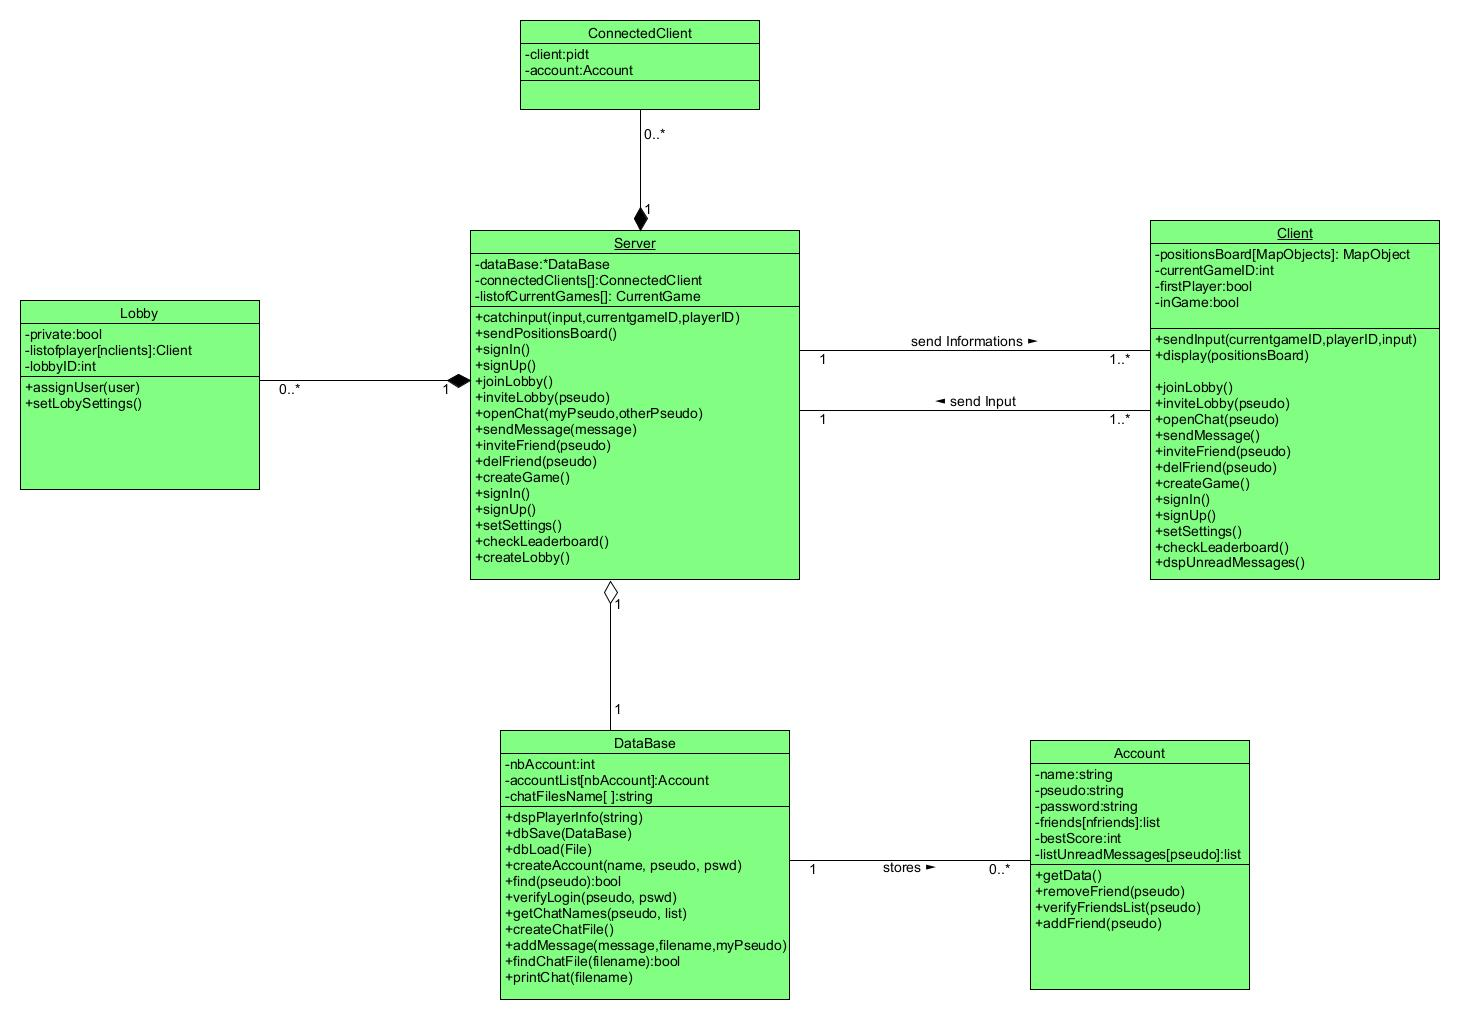
\includegraphics[width=16cm]{newSystemClassDiagram.jpg}
\caption{Diagramme de classe du système}
\label{fig:UerUseCase}
\end{figure}
\subsubsection{Server}
Le Server est notre classe principale du système. C'est la classe qui va gérer la majorité des interactions du programme. Il va servir d'intermédiaire entre le client et toutes les fonctionnalités du jeu. Pour le bon fonctionnement du jeu, cette classe devra toujours être active.\\
Parmi les fonctionnalités principales du server, on peut trouver:\\
\item- la connexion entre client et server
\item- l'interaction entre les utilisateurs
\item- la gestion des données personnelles
\item- la gestion de toutes les parties en cours
\subsubsection{Database}
La classe Database porte bien son nom puisqu'elle sauvegardera toutes les informations persistantes et nécessaires au bon fonctionnement du jeu.\\
Elle se chargera de:\\
\item- préserver et manipuler les informations personnelles relatives à chaque joueur
\item- conserver les historiques de discussions de tous les joueurs
\item- la vérification de l'existence des données
\subsubsection{Account}
Un objet Account contiendra toutes les informations relatives à un utilisateur (nom, pseudo,...). Ces informations modulables seront stockées sur la database.
\subsubsection{Lobby}
Le Lobby va servir de salle d'attente pour un ou deux joueurs avant de lancer une partie commune. L'hôte d'un lobby va pouvoir décider de son accessibilité (privé/publique).

\subsection{Besoins non fonctionnels}
\subsubsection{Connexion}
\subsubsection{Menu principal}
\subsubsection{Création de partie}
\subsubsection{Connexion}
\subsubsection{Connexion}
\subsection{Besoins non fonctionnels}

\newpage
\section{Annexes}
\subsection{ Description du diagramme use case utilisateur}

\begin{center}
\begin{longtable}{|p{1,5cm}||p{3,5cm}|p{3,5cm}|p{3,5cm}|p{3,5cm}|}
\hline
\rowcolor{green}
USE CASE   &\center{Pré-conditions}   & \hfill Post-conditions \hfill\null & Cas Général & Cas exceptionnels\\
\hline
\hline
\textbf{Sign in}      & L'utilisateur doit être enregistré dans la base de données  & L'utilisateur est connecté à sa base de données et le menu principal est affiché & L'utilisateur déjà enregistré se connecte à son compte en tapant son nom d’utilisateur et mot de passe. Le système vérifie que les données soient correctes et donne accès au compte du client.  & Si l’identifiant ou le mot de passe sont incorrectes, le système affiche un message d'erreur a l'utilisateur. \\
\hline
\hline
\textbf{Sign up}     & L'utilisateur n'est pas présent dans la base de données   & Ajout d'un compte dans la base de données et affichage du menu principal & L'utilisateur crée un compte en introduisant un pseudo et un mdp  & Si les données entrées ne respectent pas le format requis ou que le nom d'utilisateur est déjà utilisé, un message d'erreur est affiché et l'utilisateur doit recommencer l'action jusqu'à ce que ce soit valide \\

\hline
\hline
\textbf{Create game}    & L'utilisateur doit être enregistré dans la base de données  & Possibilité de sauvegarder les options requises  & L'utilisateur peut lancer une partie après avoir rempli les conditions minimales  & Néant \\
\hline
\hline
\textbf{Invite player} & L'utilisateur doit être enregistré dans la base de données   & Etablissement de la connexion via le serveur entre l’hôte et l’invité. & Inviter un joueur avec son pseudo & Invitation via pseudo qui n’existe pas. \\
\hline
\hline
\textbf{Player request}  & Recevoir une invitation via le serveur.
L'utilisateur doit être enregistré dans la base de données   & Etablissement de la connexion via le serveur entre l’hôte et l’invité.  & Accepter/ Refuser une invitation de partie  & La connexion échouera si :
Accepter une invitation dont l'hôte n’est plus connecté.
Rejoindre un salon complet. \\
\hline
\hline
\textbf{Check Leaderboard}  & L'utilisateur doit être enregistré dans la base de données   & \hfill Néant  \hfill\null &Le joueur peut consulter le classement des meilleurs scores en envoyant une requête au serveur qui va lui renvoyer les informations  & Néant \\
\hline
\hline
\textbf{View friend list }   & L'utilisateur doit être enregistré dans la base de données   & Néant  & Consultation de liste d'ami dans la base de données. & Néant \\
\hline
\hline
\textbf{Chat}     & L'utilisateur doit être enregistré dans la base de données   & Le serveur effectue les liaisons entre les utilisateurs  & Envoyer et recevoir des messages avec n'importe quel pseudo.  & Néant \\
\hline
\hline
\textbf{Add friend}    & L'utilisateur doit être enregistré dans la base de données   & Si invitation acceptée, ajout d'amis dans la base de donnée (bidirectionnel).  & Entrer le pseudo d’un ami. Le système va rechercher dans la base de données si le pseudo existe et l’ajouter.  & Ajouter un ami qui n’existe pas (affiche une erreur).\\
\hline
\hline
\textbf{Delete friend}    & L'utilisateur doit être enregistré dans la base de données et avoir au moins un ami.   & Suppression d’amis(de la liste d’amis) de la base de données.  & Entrer le pseudo d’un ami. Le système va rechercher dans la base de données si le pseudo existe et le supprimer.  & Supprimer un ami qui n’existe pas (affiche une erreur). \\
\hline
\hline
\textbf{Settings}     & L'utilisateur doit être enregistré dans la base de données   & Mise à jour des changements  & L'utilisateur modifie des parametres de son profil de l'affichage ou du son  & Néant\\
\hline
\hline
\textbf{Ship’s controls}  & Charger une partie/créer une partie.   & Actualisation de l’état de jeu.  & Bouger, tirer recevoir des bonus.  & Néant\\
\hline
\hline
\textbf{Leave party}      & Être en train de jouer   & Retour au menu principal  & Le joueur arrête la partie en cours.  & Néant\\
\hline
\hline
\textbf{Help}      & Etre connecté   & Néant  & Les règles principales du jeu sont affichées au joueur & Néant\\
\hline
\hline
\textbf{Leave game}      & Etre connecté   & Fermeture du jeu  & L'utilisateur est connecté et veut quitter le jeu  & L'utilisateur est connecté et force sa sortie du jeu (CTRL+C, ...)\\
\hline
\end{longtable}
\end{center}


\end{document}
